%This is a template for producing reports for "Dagstuhl Reports".
%See dagrep.pdf for furhter information.

\documentclass[a4paper,UKenglish]{dagrep}
  %for A4 paper format use option "a4paper", for US-letter use option "letterpaper"
  %for british hyphenation rules use option "UKenglish", for american hyphenation rules use option "USenglish"
  %for section-numbered lemmas etc., use "numberwithinsect"

\usepackage{microtype}%if unwanted, comment out or use option "draft"
\usepackage{biblatex}
\usepackage{float}
\usepackage{comment}
\usepackage[many]{tcolorbox}

%\bibliographystyle{plain}%the recommended bibstyle
\bibliography{bibliography.bib}

\subject{Performance engineering}
\title{Patterns and anti-patterns of efficient software}
\titlerunning{Patterns and anti-patterns}%optional

\author[1]{Oscar Palm}
%\author[2]{Joan R. Access}
\affil[1]{Chalmers University of Technology, Sweden
  \texttt{nilsosc@chalmers.se}}
%\affil[2]{Department of Informatics, Dummy College Address, Country
%  \texttt{access@dummycollege.org}}
\authorrunning{Oscar Palm}%optional

%\keywords{Sample Article, Dagstuhl Seminar, Dagstuhl Perspectives Workshop}%optional

\keywords{Performance Engineering, Software Engineering}

%Organizer macros:%%%%%%%%%%%%%%%%%%%%%%%%%%%%%%%%%%%%%%%%%%%%%%%%%%%%%
\seminarnumber{11013}
%\semdata{03.--07.~January, 2011 -- \url{http://www.dagstuhl.de/11013}}

%%%%%%%%%%%%%%%%%%%%%%%%%%%%%%%%%%%%%%%%%%%%%%%%%%%%%%%%%%%%%%%%%%%%%%%

%Dagstuhl editorial office macros:%%%%%%%%%%%%%%%%%%%%%%%%%%%%%%%%%%%%%
\volumeinfo%(easychair interface)
  {Oscar Palm}%editors
  {1}%number of editors
  {Special Topics in Software Engineering}%event
  {1}%volume
  {2025}%issue
  {1}%starting page number
\DOI{10.4230/DagRep.1.1.1}%(DagRep.<issue no>.<volume no>.<firstpage>)
%%%%%%%%%%%%%%%%%%%%%%%%%%%%%%%%%%%%%%%%%%%%%%%%%%%%%%%%%%%%%%%%%%%%%%%



\newtcolorbox{patt}[0]{enhanced,colback=blue!10!white,colframe=blue!75!black,width=0.8\textwidth}
\newtcolorbox{apatt}[0]{enhanced,colback=red!10!white,colframe=red!75!black,width=0.8\textwidth}

\newcommand{\pattern}[6]{
\begin{center}
  \begin{patt}
    \begin{description}
      \item[Pattern Name:]#1
      \ifthenelse{#2 = 0}{~}{\item[Also Known As:]#3}
      %\item[Most Frequent Scale:] #4
      \item[Issue To Fix:]#5
    \end{description}
  \end{patt}
\end{center}
  \textbf{Background}\\#6

  }
\newcommand{\antipattern}[7]{
  \begin{center}
    \begin{apatt}
      \begin{description}
        \item[Anti-Pattern Name:]#1
        \ifthenelse{#2 = 0}{~}{\item[Also Known As:]#3}
        %\item[Most Frequent Scale:] #4
        \item[Solution Name:]#5
      \end{description}
    \end{apatt}
  \end{center}
  \textbf{Background}\\#6
  ~\\\\
  \textbf{Solution}\\#7
  }

\begin{document}

\maketitle





%\newpage
\section{Introduction}
An anti-pattern, as described by Brown et al. \cite{brown1998antipatterns}, is a method of recognising recurring problems in software engineering, and providing a general solution and a common vocabulary for identification and solving these recurring problems. This chapter intends to present and discuss anti-patterns within the field of performance engineering, as well as the common solutions, or patterns, for problems within the field.
For the readers' benefit, patterns and anti-patterns have been grouped into categories, and in some cases similar patterns have been combined.

To present the patterns in a structured way, a modified version of the template presented  by Brown et al. in their book AntiPatterns \cite{brown1998antipatterns}, has been used.


The purpose of this chapter is to understand common performance issues in software engineering, and how these issues can be solved through planning and good design. The patterns will also help understand common issues within the field, helping maintainer find problems, and understand ways of solving them.

\subsection{Taxonomy of patterns}
The patterns  and anti-patterns have been divided into several categories, representing during which type of work the pattern is useful, or the anti-pattern is commonly found. Since more patterns were found than can be discussed in a single chapter, a list of found patterns and anti-patterns can be found at the start of each category.. %A list of All found Patterns and Anti-patterns relating to, and which literature more can be read about them in, can be found in  Tables \ref{tab:patterns} and \ref{tab:antipatterns}.

The top-level categories, as seen in Figure \ref{fig:overview}, does not take into account similarities between patterns, but is only a grouping of the problems a pattern intends to solve. Some patterns in different categories can therefore be similar to each other. An example of this is the Priority Queue and the Competing Consumers patterns.

Further, some categories have themselves been divided into sub-categories. More information about these divisions will be presented within the relevant categories.

\begin{figure}
\centering
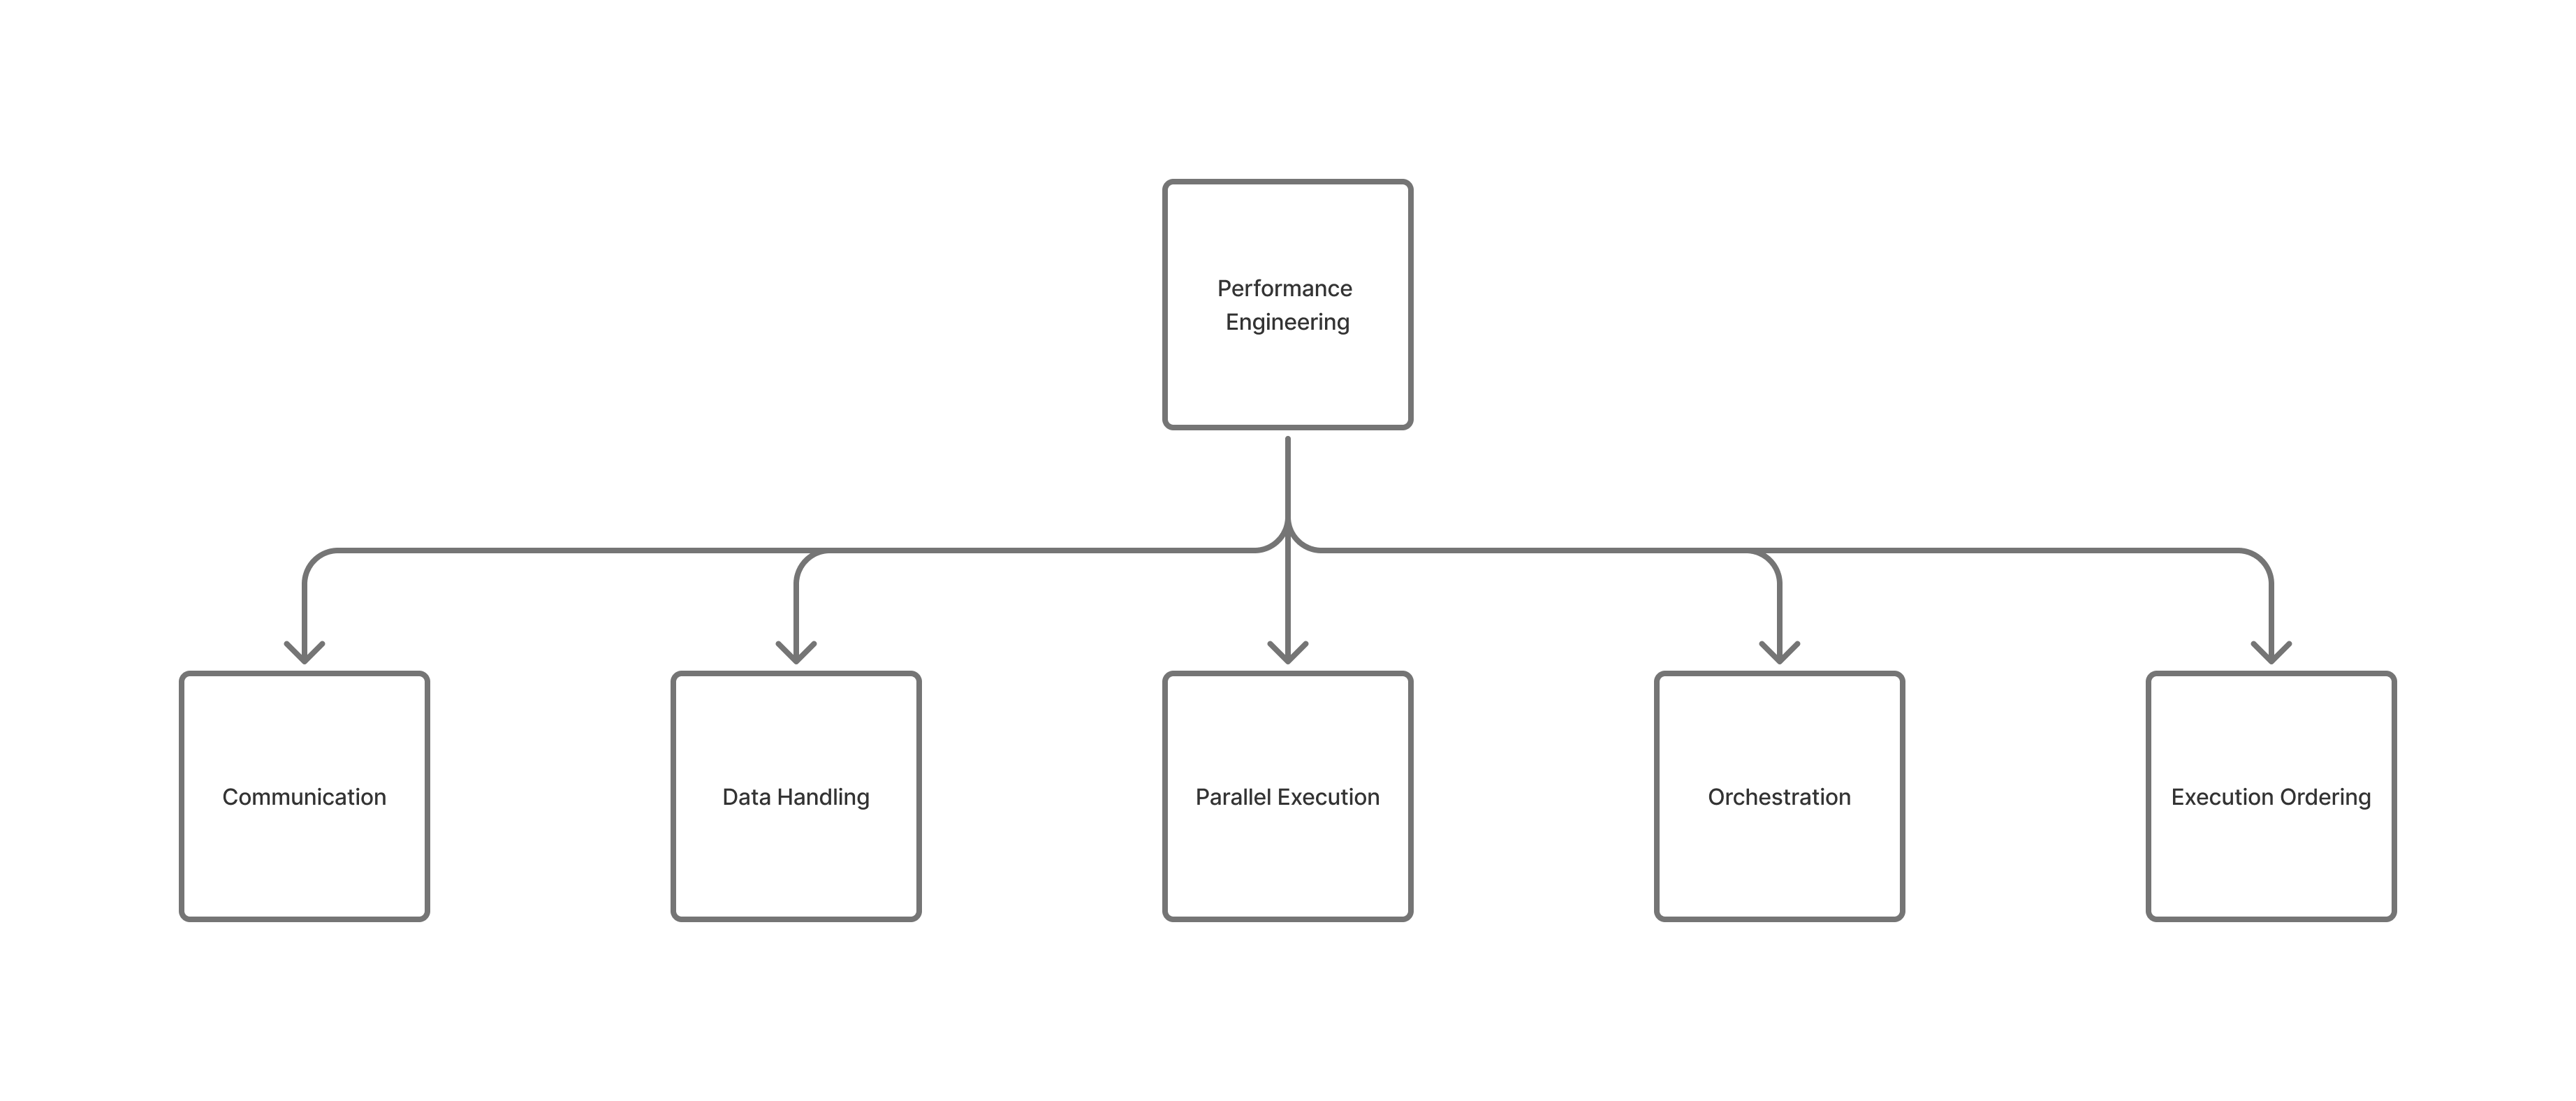
\includegraphics[width=.7\textwidth]{presentation/figures/overview}
\caption{Overview of categories of patterns and anti-patterns}
\label{fig:overview}
\end{figure}




%\textbf{Notes:} For each category / chapter I have a list of all patterns and anti-patterns I will write about, and which source(s) it is described in. In total it's slightly above 50 patterns, but I intend to group several similar ones into the same pattern, similar to the patterns presented in the book Antipatterns (see \cite{brown1998antipatterns}). e.g. Empty semi-truck and round tripping have a big overlap.


\section{Communication}
Sending and receiving of data between different components is something most computer programs does, logically several patterns and antipatterns discuss the various problems relating to this communication.

The patterns and antipatterns can be divided into two categories, one discussing performance and performance issues when communicating within the same application, while the category discusses performance issues when communicating between different applications.

\begin{table}[H]
	\begin{tabular}{c|ccc}
		Name                       & Type    & Category           & Source                                    \\\hline
		Asynchronous Request-Reply & Pattern & Internal Communication      & \cite{microsoft2024performanceefficiency} \\
		Backends for Frontends     & Pattern & Network Communication      & \cite{microsoft2024performanceefficiency} \\
		Circuit Breaker            & Pattern & Network Communication      & \cite{microsoft2024performanceefficiency} \\
		Queue-Based Load Leveling  & Pattern & Network Communication      & \cite{microsoft2024performanceefficiency} \\
		Choreography               & Pattern & Internal Communication      & \cite{microsoft2024performanceefficiency} \\
		Sidecar                    & Pattern & Network Communication      & \cite{microsoft2024performanceefficiency} \\
		Synchronous I/O                   & Anti-pattern & Network Communication      & \cite{MicrosoftAntipatterns}                            \\
		Falling Dominoes                  & Anti-pattern & Network Communication      & \cite{more_se_antipatterns}                             \\
		Empty Semi Truck                  & Anti-pattern & Network Communication      & \cite{more_se_antipatterns},\cite{detect_antipatterns}  \\
		Round-tripping                    & Anti-pattern & Network Communication      & \cite{tate2002bitter}                                   \\
		Busy Database                     & Anti-pattern & Network Communication      & \cite{MicrosoftAntipatterns}                            \\
		Busy Front End                    & Anti-pattern & Network Communication      & \cite{MicrosoftAntipatterns}                            \\
		Chatty I/O                        & Anti-pattern & Network Communication      & \cite{MicrosoftAntipatterns}                            \\
		Retry Storm                       & Anti-pattern & Network Communication      & \cite{MicrosoftAntipatterns}                            \\
		Too many Remote Calls             & Anti-pattern & Network Communication      & \cite{framework_assessing_antipatterns}                 \\
		Tower of Babel                    & Anti-pattern & Internal Communication      & \cite{more_se_antipatterns},\cite{detect_antipatterns}  \\
		Improper Instantiation            & Anti-pattern & Internal Communication      & \cite{MicrosoftAntipatterns}                            \\
		Excessive Dynamic Allocation      & Anti-pattern & Internal Communication      & \cite{detect_antipatterns}                              \\
		Aggressive Loading of Entities    & Anti-pattern & Internal Communication      & \cite{framework_assessing_antipatterns}                 \\
		Circuitous Treasure Hunt          & Anti-pattern & Network Communication      & \cite{detect_antipatterns}                              \\
	\end{tabular}
	\caption{All found Patterns and Anti-patterns relating to network communication}
	\label{tab:patterns}
\end{table}


\subsection{Network Communication}
Following are patterns relating to different applications communicating, both over networks, but also within the same computer. Most of these patterns discuss how to efficiently use relevant I/O devices.

Since sending and receiving of data can be time consuming when communicating between computers, the communication itself can become a performance issue. Many patterns and anti-patterns discuss this communication between computers and we can roughly divide them into two groups, where one group discusses the data in each request, and the other group discusses how the requests themselves can be handled more efficiently.

\subsubsection{Data Handling in Network Communication}

For the first group of patterns, an example is the Empty Semi Truck anti-pattern, which discusses how what logically might be several distinct requests sometimes can be combined into one request, to limit the idling time of a client.

\antipattern{Empty Semi Truck \cite{more_se_antipatterns,detect_antipatterns}}{0}{}{}{Batching of requests}{
	This antipattern occurs when a client sends more requests than necessary, slowing down execution because of idling time waiting for the unnecessary amount of responses \cite{detect_antipatterns}.

	Empty Semi Trucks are caused by one of two main issues; a poorly written interface, or an inefficient use of the bandwidth \cite{more_se_antipatterns}.

}{
	For the first case, a poorly written interface, allowing for coupling of several request into one helps decrease the amounts of requests needed \cite{detect_antipatterns}. Depending on what currently is forcing the client to send multiple requests, what needs to be rewritten can change, but examples can be allowing for clients to fetch entire objects, instead of separate requests for different parts of it, or allowing the fetching of several objects at once.

	If the problem instead is using the bandwidth inefficiently, we can instead use batching to combine several requests into one \cite{detect_antipatterns}. This helps lower the overhead of sending and receiving several messages.
}

\subsubsection{Request Handling in Network Communication}
The other group of patterns and anti-patterns related to network communication discuss how to handle requests; is it possible to perform other tasks while waiting for responses? Can we send multiple requests at once? Many of the patterns and anti-patterns discuss using asynchronous computing to better utilise computing resources.

Commonly, software is written synchronously, meaning the previous instruction needs to complete before continuing execution; with network communication however, the time of some instructions may take a very significant amount of time. Several Patterns and Anti-patterns discuss ways of utilising the computer to avoid idly waiting for these requests to complete.


\antipattern{Synchronous I/O \cite{MicrosoftAntipatterns}}{0}{}{}{Asynchronous messaging}{The program is blocked by a synchronous I/O call. No useful work is completed while the I/O operation completes. Often this occurs while requesting data from web services or fetching data from discs.}{ Convert the synchronous I/O operation to an asynchronous one, if possible, execution of other operations can continue while the resulting I/O action is completing. While this does not always solve the problem; some times data from the I/O operation is needed to continue, often times the result from such operations are not used, think storing data; in which case synchronicity is consuming time unnecessarily. }

\pattern{Asynchronous Request-Reply \cite{microsoft2024performanceefficiency}}{1}{Polling \cite{Mohamed-Ali2025shortpolling}}{ }{Synchronous web calls leading to unnecessarily long load times.}{
	In modern web applications, it's common to use data or services from external APIs, such as to show advertisement, handle authentication, or to access certain data. Instead of the server not returning until these requests have been completed and the result ready, http polling can be used.

	With polling, the server responds immediately with status 202 accepted. When the client later needs to access the result, it polls the server, which instead can either return code 302, value found, and redirect to where the result can be found, or code 200, the result is not ready yet, after which the client can poll again later.

	While this in itself might not mitigate the problem with long wait times, if the client is structured smartly, data can be requested before it is needed, freeing up the client to perform other tasks while the request is completing.
}


\subsection{Internal communication}
These patterns relate to issues regarding communication between different modules, classes, functions, or other divisors within a software system.

Since the communication is most likely happening between systems with smaller request latency, the main focus is not the requests any more, but rather what data is sent. The shorter messaging time means performance issues more likely arise from handling the requests rather than waiting for the requests to complete.

While some of the patterns and anti-patterns, such as Tower of Babel, discuss minimising the cost of communication in different ways, others instead recognise the limits of vertical scalability.

Patterns, such as the Choreography pattern, instead discuss ways of offloading some of the requests to other instances of the same service.

Both of these types of improving efficiency of the software is necessary. When only focusing on horizontal scaling of systems, inefficient use of system resources might still be a problem. This might make larger requests bottleneck the system. Likewise if only focusing on vertical scaling, the hardware used limits the efficiency of a system heavily.


\antipattern{Tower of Babel \cite{more_se_antipatterns, detect_antipatterns}}{0}{}{Most frequent}{Minimise parsing and translation}{
	When sending data between components, it is common to translate said data into common formats, such as JSON, XML, or CSV. It is however common for both the receiving and sending component to use its own internal representation of the data, sometimes even the same internal representation in both components.

	This conversion between different data formats can be costly, especially when not only two components are communicating, but rather a chain of several components.
}{
	Using the fast path performance pattern \cite{more_se_antipatterns} we notice which paths are in need of streamlining. For these paths, we rewrite the code to minimise the amount of translation between data representations.

	When data is sent within the system, make sure all parts use the same internal representation, instead of translation between different internal representations and / or export formats such as XML \cite{more_se_antipatterns}.

}

\pattern{Choreography \cite{microsoft2024performanceefficiency}}{0}{}{}{When a system is under heavy use, the need for scalability becomes more prominent. With direct communication between different services within the system, it can be hard to scale the system efficiently \cite{microsoft2024performanceefficiency}.

	Instead routing requests through an orchestrator requires a very complex architecture and often relies on custom third party software, such as kubernetes.}{
	Instead of using direct communication or orchestrators, a queue of tasks can be used. With a queue based system, services can poll the queue to see if the task is something they can process or not.

	This pattern is similar to the Competing Consumers pattern \cite{microsoft2024performanceefficiency}, and Worker Pool pattern\cite{zepeda2024workerpool}, with the distinction of each worker being able to represent a different service. This means that while a worker in the worker pool is identical to all other workers, in the choreography pattern, each service can be either different instances of the same service, or its own distinct service.


}



\section{Data handling}

This group of patterns are related to access of, and storage of, data. Whether it is related to data stored in files on the disk, or in a database, these patterns help you manage access to it.

Similar to network communication, accessing of data is time consuming, especially when said data is not stored  locally.

\begin{table}[H]
	\begin{tabular}{c|ccc}
		Name                       & Type    & Category           & Source                                    \\\hline
		Cache-aside                & Pattern & Data Handling      & \cite{microsoft2024performanceefficiency} \\
		Claim Check                & Pattern & Data Handling      & \cite{microsoft2024performanceefficiency} \\
		Event Sourcing             & Pattern & Data Handling      & \cite{microsoft2024performanceefficiency} \\
		Index Table                & Pattern & Data Handling      & \cite{microsoft2024performanceefficiency} \\
		Materialized View          & Pattern & Data Handling      & \cite{microsoft2024performanceefficiency} \\
		No Caching                        & Anti-pattern & Data Handling      & \cite{MicrosoftAntipatterns}                            \\
		Extraneous Fetching               & Anti-pattern & Data Handling      & \cite{MicrosoftAntipatterns}                            \\
		Monolithic Persistence            & Anti-pattern & Data Handling      & \cite{MicrosoftAntipatterns}                            \\
	\end{tabular}
	\caption{All found Patterns and Anti-patterns relating to data handling}
	\label{tab:patterns}
\end{table}

\pattern{Cache-aside \cite{microsoft2024performanceefficiency}}{0}{}{}{Accessing data from a database takes time, storing the data locally is not an option either since data in the database might get updated over time.}{
	Caching is used to improve the performance of an application by storing commonly used information in a server temporarily instead of always requesting the data from an external party \cite{wessels2001webcaching}.

	It can be hard to manage a cache, since data over time becomes outdated, or stale, without the client knowing. This issue of knowing when to update the cache is a challenge in development of distributed systems \cite{microsoft2024performanceefficiency}.

	Instead of loading data from the database, or other similar services, this pattern suggest implementing a cache, where each data request first checks if the data exist in the cache before requesting data externally \cite{microsoft2024performanceefficiency}.

	When data is being fetched, it is also added to the cache in case it is needed later on \cite{microsoft2024performanceefficiency}.
}







\section{Parallel Execution}

Parallelism is a tool often used to increase performance  of applications\cite{mak1997parallelism}, but if used incorrectly, its benefits might not come into effect and in the worst case, a performance decrease can even be seen.




\begin{table}[H]
	\begin{tabular}{c|ccc}
		Name                       & Type    & Category           & Source                                    \\\hline
		Competing Consumers        & Pattern & Parallel Execution & \cite{microsoft2024performanceefficiency} \\
		Concurrent Processing Systems     & Anti-pattern & Parallel Execution & \cite{detect_antipatterns}                              \\
		''Pipe and Filter'' Architectures & Anti-pattern & Parallel Execution & \cite{detect_antipatterns}                              \\
		One-Lane Bridge                   & Anti-pattern & Parallel Execution & \cite{detect_antipatterns}                              \\
		More is Less                      & Anti-pattern & Parallel Execution & \cite{detect_antipatterns}                              \\
	\end{tabular}
	\caption{All found Patterns and Anti-patterns relating to parallel execution}
	\label{tab:patterns}
\end{table}

The More is less anti pattern is a great example of how parallelism can hurt the performance of an application because of the extra overhead added when making a task parallelised.


\antipattern{More is less \cite{detect_antipatterns}}{0}{}{}{Less forking.}{A process creating sub-processes to perform parallel execution in some cases ends up spending more time handling threads than performing actual work.}{
	The solution to execution time slowing because of "over-parallelising" is to limit the amount of allowed processes. Since the limits of when thrashing occurs is dependent on both hardware and the parallelised software \cite{denning1968thrashing}, we test the specific combination of hardware and software, to quantify which threshold for amount of processes where thrashing occurs \cite{detect_antipatterns}.

	Based on the results from this test, we can then decide a limit for amount of processes, or in case of the architecture not meeting performance goals, modify the architecture until performance goals are met.
}

Even when parallelism is implemented in a way, helping the performance of an application, it is easy to create threads with uneven workloads, leading to large parts of the theoretically parallelisable application being executed sequentially. The Competing Consumers pattern discusses how this problem can disappear, by modifying the architecture of our system.

\pattern{Competing Consumers \cite{microsoft2024performanceefficiency}}{1}{Worker Pool pattern \cite{zepeda2024workerpool}}{}{When a module in a system sees heavy use, and some requests take a long time to process, it might be frustrating for users when a seemingly simple request takes much longer than usual just because their task got assigned the ''wrong'' thread.}{
	By using a message queue, several instances of the service can work on the tasks simultaneously. This allows for easier horizontal scaling of the service, since instances can be created or removed without interrupting the rest of the system.

	Usage of the message queue also improves reliability since a failure in a consumer, or worker, does not mean all pending messages will be lost, unlike with direct communication between producer and consumer \cite{microsoft2024performanceefficiency}.

	Usage of this pattern also removes the issue of uneven workload distribution, since all processes share the same backlog of tasks.
}


\section{Orchestration}

For hosting of services, it is common to use orchestrators to help divide and manage their resources. When the amount of users of a service grows, it is also common to have several instances of a service, either to share the processing load, or to minimise access time by distributing instances over different servers spread across the globe. Chaotic session management is an anti-pattern that might appear when using several instances of an application without accounting for the separate memory of different instances.

When orchestrating systems, comprised of several different services, or instances of the same service, there is also a need to allow clients to connect to all of these, it can be hard to remember which service does what, or to know which instance of a service to connect to. The Gateway Routing Pattern helps balance loads and connect clients to relevant servers without the need to understand the internal architecture.

\begin{table}[H]
	\begin{tabular}{c|ccc}
		Name                       & Type    & Category           & Source                                    \\\hline
		Gateway Aggregation        & Pattern & Orchestration      & \cite{microsoft2024performanceefficiency} \\
		Gateway Offloading         & Pattern & Orchestration      & \cite{microsoft2024performanceefficiency} \\
		Gateway Routing            & Pattern & Orchestration      & \cite{microsoft2024performanceefficiency} \\
		Health Endpoint Monitoring & Pattern & Orchestration      & \cite{microsoft2024performanceefficiency} \\
		Scheduler Agent Supervisor & Pattern & Orchestration      & \cite{microsoft2024performanceefficiency} \\
		Sharding                   & Pattern & Orchestration      & \cite{microsoft2024performanceefficiency} \\
		Throttling                 & Pattern & Orchestration      & \cite{microsoft2024performanceefficiency} \\
		Chaotic Session Management        & Anti-pattern & Orchestration      & \cite{tate2002bitter}                                   \\
		Noisy Neighbor                    & Anti-pattern & Orchestration      & \cite{MicrosoftAntipatterns}                            \\
		Traffic Jam                       & Anti-pattern & Orchestration      & \cite{detect_antipatterns}                              \\
	\end{tabular}
	\caption{All found Patterns and Anti-patterns relating to orchestration}
	\label{tab:patterns}
\end{table}


\antipattern{Chaotic session management \cite{tate2002bitter}}{0}{}{}{
	Dispatching with session affinity}{When managing sessions over several different instances of a system, the session of a user in one instance is not immediately transferred to other instances, and we do not always want to send a user's session information to all instances of the system.

	To the user however, if the next request they send are routed to another instance of the service, it will look as if their session has been terminated. There needs to exist a better way to handle sessions in a system with multiple instances.
}{
	One easy solution to this problem is to always dispatch requests from the same user to the same instance; if the user always communicates with the same server, the distributedness of the architecture is hidden \cite{tate2002bitter}.

	Some issues still persist with this solution however. If an instance fails, all users assigned to that instance will lose their session. Since one of the major benefits of having several instances of a system is that  (hopefully) the reliability is higher, because other instances of the service can replace failing ones; this is a major flaw in the solution. However, other solutions which mitigate this issue comes with performance penalties \cite{tate2002bitter}, meaning this is still one of the better solutions to the problem.
}

\pattern{Gateway Routing \cite{microsoft2024performanceefficiency}}{0}{}{}{With a distributed system, it can be tricky remembering which API does what, and the name of the services.

	It can also be tricky knowing how many instances of a service exists and which one to connect to. }{
	By having a gateway service, that routes each request to the relevant service, and instance of that service, clients need only connect to a single API, hiding implementation logic, and exact details of which instance the user is connected to \cite{microsoft2024performanceefficiency}.

	Usage of this pattern allows for easy horizontal scaling of services, as well for increased reliability, since after a failure in one of the instances, requests can be routed through the gateway to other instances, without the need for clients to repeat the request.

	It however introduces a single point of failure, if an issue happens in the gateway, access to all services are lost \cite{microsoft2024performanceefficiency}. Similarly since the gateway is a service in itself, it can also be overloaded; if it is not fast enough, it can itself become a performance issue \cite{microsoft2024performanceefficiency}.
}



\section{Execution Ordering}

The order different tasks are executed in can affect the performance of an application, if the tasks are executed in a bad order, a parallelised program can be forced to execute partly serialized.

While tasks such as garbage collection and backupping are important, they take time. A Website that does not consider its execution order might schedule a system backup while a system tries accessing a web page, severely worsening the load time of the page, possibly losing customers.

The Priority Queue pattern discusses how tasks can be given different priorities to help manage the order they will be executed.

\begin{table}[H]
	\begin{tabular}{c|ccc}
		Name                       & Type    & Category           & Source                                    \\\hline
		Priority Queue             & Pattern & Execution Ordering & \cite{microsoft2024performanceefficiency} \\
		Publisher / Subscriber     & Pattern & Execution Ordering & \cite{microsoft2024performanceefficiency} \\
		Bad Workload Management           & Anti-pattern & Execution Ordering & \cite{tate2002bitter}                                   \\
	\end{tabular}
	\caption{All found Patterns and Anti-patterns relating to execution ordering}
	\label{tab:patterns}
\end{table}

\pattern{Priority Queue \cite{microsoft2024performanceefficiency}}{0}{}{}{
	Tasks handled by a system is not all of the same level of importance, having critical tasks delayed, because of relatively unimportant tasks in the queue, can cost a lot of money for companies, or in worst case lead to death, in case of healthcare software.
}{
	By assigning each task a priority, we can make sure that critical tasks are handled before not as critical tasks. There's two main ways of creating a priority queue, either there's one list of all queued tasks, where each task is given a priority and the queue sorts its item after priority The other option is to create one queue per priority level, making sure the highest-level queue is empty before working on tasks from lower priorities \cite{microsoft2024performanceefficiency}.

	While a single queue works fine for most cases, it can become slow to add tasks when the queue grows large, as it needs a way to sort itself.

	Using multiple queues has many benefits; for one, the existence of several queues means instances of a service can be assigned different priority levels, making sure that while the higher priority queue still have priority, the lower priority tasks still resolves \cite{microsoft2024performanceefficiency}.
}




\section{Miscellaneous}
Some patterns and  anti-patterns doesn't fit into a grouping of problem areas as well as others. Since these are still important to consider while developing and refactoring they are still included in the chapter.


\begin{table}[H]
	\begin{tabular}{c|ccc}
		Name                       & Type    & Category           & Source                                    \\\hline
		Federated Identity         & Pattern & Miscellaneous      & \cite{microsoft2024performanceefficiency} \\
		Performance Afterthoughts         & Anti-pattern & Miscellaneous      & \cite{tate2002bitter}                                   \\
		Blob                              & Anti-pattern & Miscellaneous      & \cite{detect_antipatterns},\cite{brown1998antipatterns} \\
		Extensive Processing              & Anti-pattern & Miscellaneous      & \cite{detect_antipatterns}                              \\%(Not sure this can classify)\\
		The Ramp                          & Anti-pattern & Miscellaneous      & \cite{detect_antipatterns}                              \\
	\end{tabular}
	\caption{All found Patterns and Anti-patterns relating to miscellaneous.}
	\label{tab:antipatterns}
\end{table}

While most patterns and anti-patterns discussed focus on the execution time of application, other factors also affect the performance of an application.  The Blob anti-pattern is one of these, discussing how poorly written code can affect the memory usage of applications \cite{brown1998antipatterns}.
\antipattern{Blob \cite{brown1998antipatterns,detect_antipatterns}}{1}{The God Class \cite{detect_antipatterns}}{}{}{The Blob is a class which does more than it is supposed to, instead of a system containing classes with data, and functionality related to the data, systems with a blob generally contain data classes, with limited functionality, and a larger "Blob" which performs most of the operations these data classes should include.

	From a performance perspective, Blobs are concerning since the loading of large classes is memory heavy, meaning loading all data for the Blob, every time a simple operation is performed, can slow execution time \cite{brown1998antipatterns}.
}{
	Since the performance degradation is due to excessive loading of data into memory, the solution is to lower the amount of data loaded into memory. To do this, functionality regarding data from other classes should be moved to those classes \cite{detect_antipatterns}.

	It can also help to remove associations to other classes, moving those associations to other classes instead \cite{brown1998antipatterns}.
}







\section{Conclusion}
This chapter has discussed various types of patterns  as well as how they can be applied in real-world scenarios. Where different anti-patterns can be found and how to deal with them have also been discussed.

While most patterns found are related to development of distributed systems, such as web applications, the same patterns can also be applied to other types of system.

The chapter also provides a common vocabulary to discuss problems and problem solutions within performance engineering, helping developers communicate issues and teams of developers understand the choices made by other people. While patterns do not always provide the best solution for a specific case, the generality and widespread solution description helps create a maintainable code base.

A recurring theme throughout the chapter is the effect of performance bottlenecks. The bottlenecks are created by inefficient communication, inefficient resource use, or executing tasks without prioritisation. Many of these patterns do not focus on improving the code, but rather on balancing the work, and utilising the computer's resources in a better way.

Many of the anti-patterns discussed instead describe how laziness during planning can lead to problems such as Blobs \cite{brown1998antipatterns,detect_antipatterns} or Synchronous I/O \cite{MicrosoftAntipatterns}, which in turn creates issues for the performance of an application.

\printbibliography




\end{document}
